\subsection{Role Assignment}
As aforementioned role assignment was predefined for the robot set. In the project three robots were given static characteristics, these characteristics were defined based on robot attributes. The simplified set of attributes taken into consideration were maneuverability and robot height. These attributes corresponded to terrain traversability, the terrain was indexed as follows: 0 - open terrain, 1 - ramp, 2 - short tunnels, and 3 - tall tunnels. Given the set of robots and attributes capabilities were defined. Robot 1 (Youbot) could traverse terrain 0, 2, and 3. Robot 2 (Rosbot) could traverse terrain 0, 1, and 3. Robot 3 (Husky) could traverse terrain all terrains in the terrain set, the robots and terrain is illustrated in figure \ref{fig:map}.


\begin{figure}
    \centering
    \begin{subfigure}[b]{0.15\textwidth}
        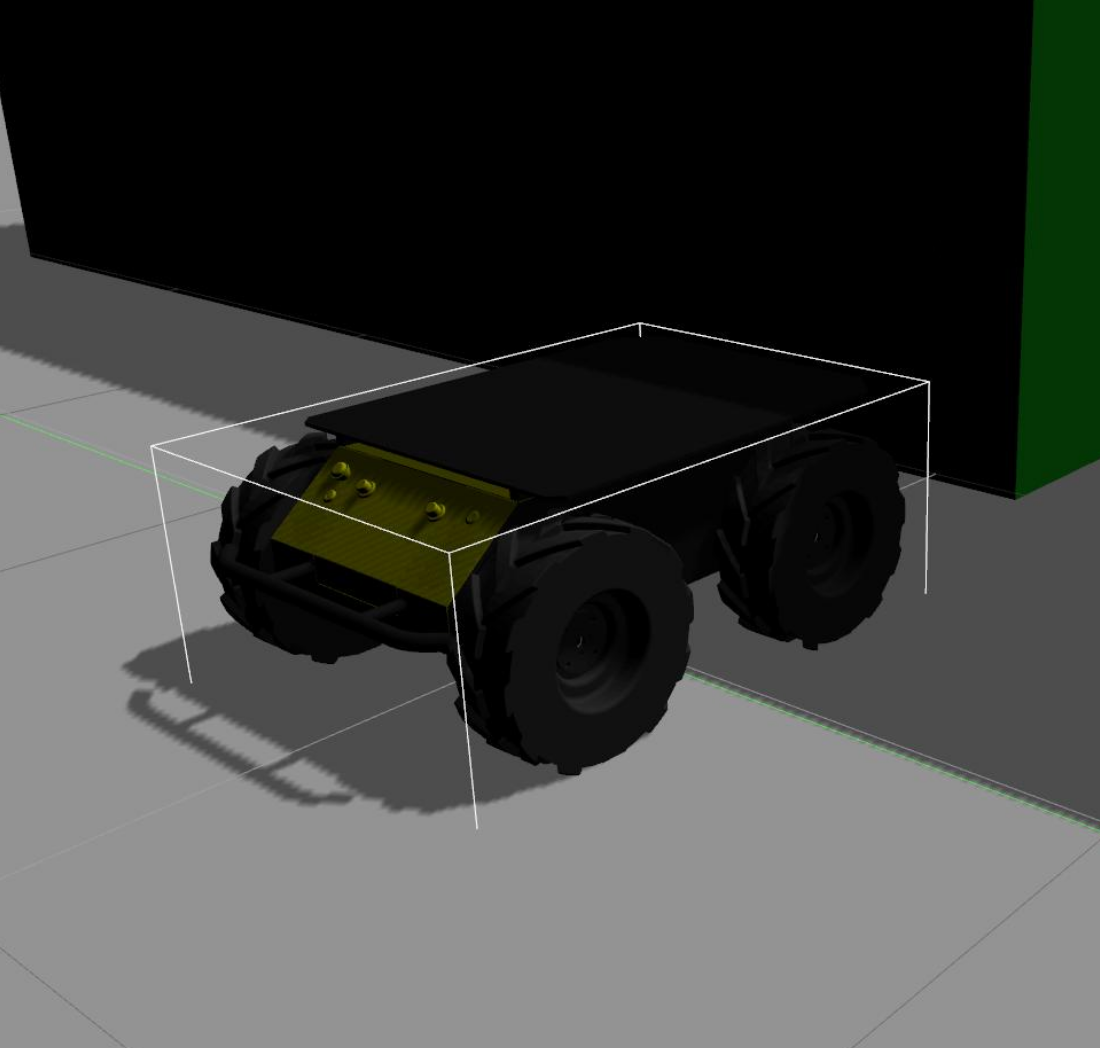
\includegraphics[width=\textwidth]{bot1}
        \caption{Husky}
        \label{fig:bot1}
    \end{subfigure}
    \begin{subfigure}[b]{0.15\textwidth}
        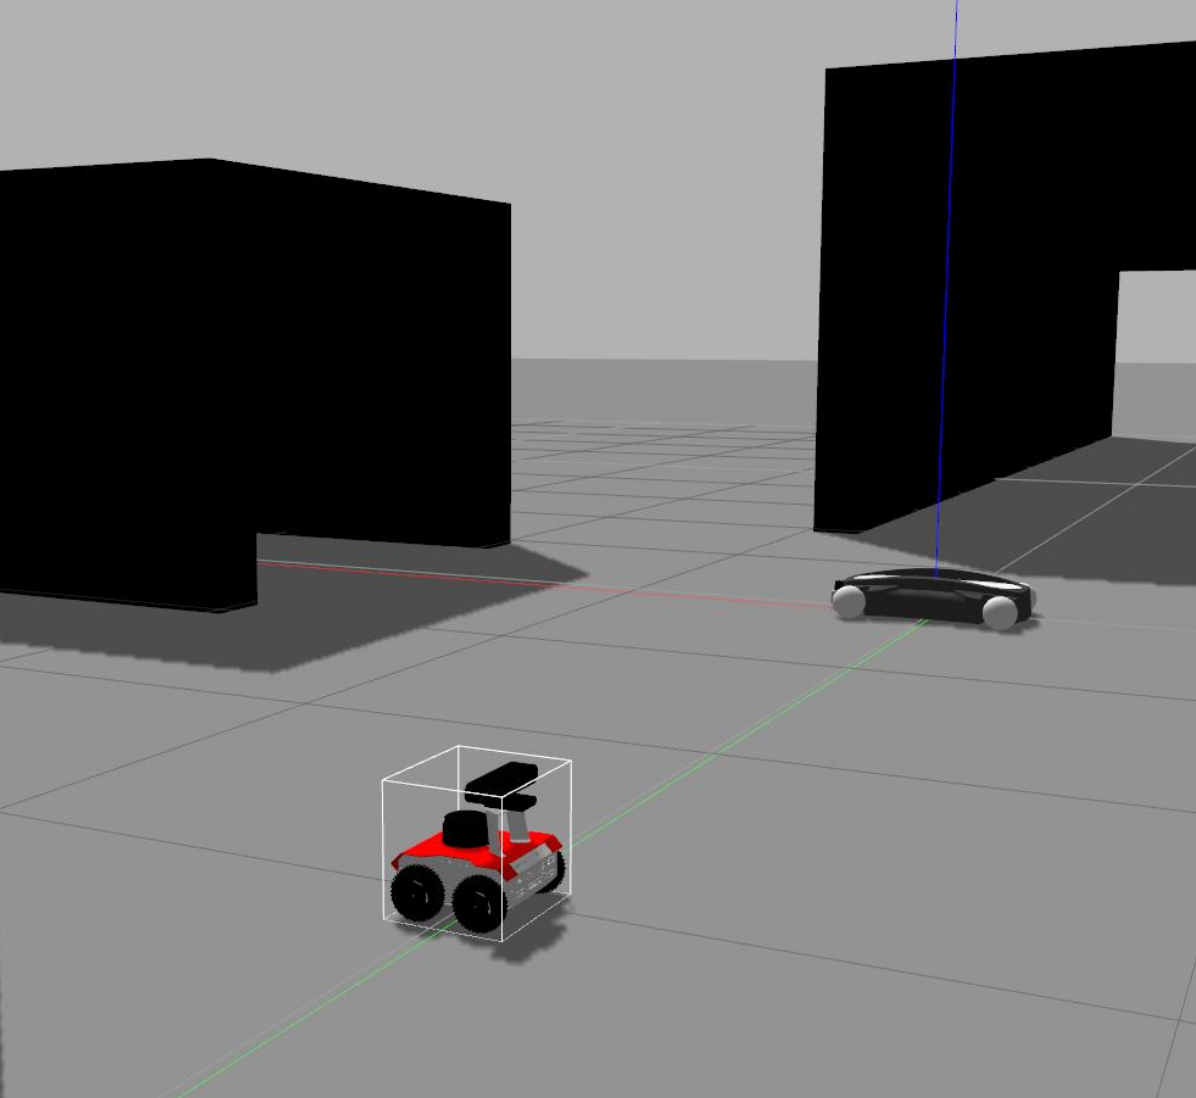
\includegraphics[width=\textwidth]{bot2}
        \caption{Rosbot}
        \label{fig:bot2}
    \end{subfigure}
    \begin{subfigure}[b]{0.15\textwidth}
        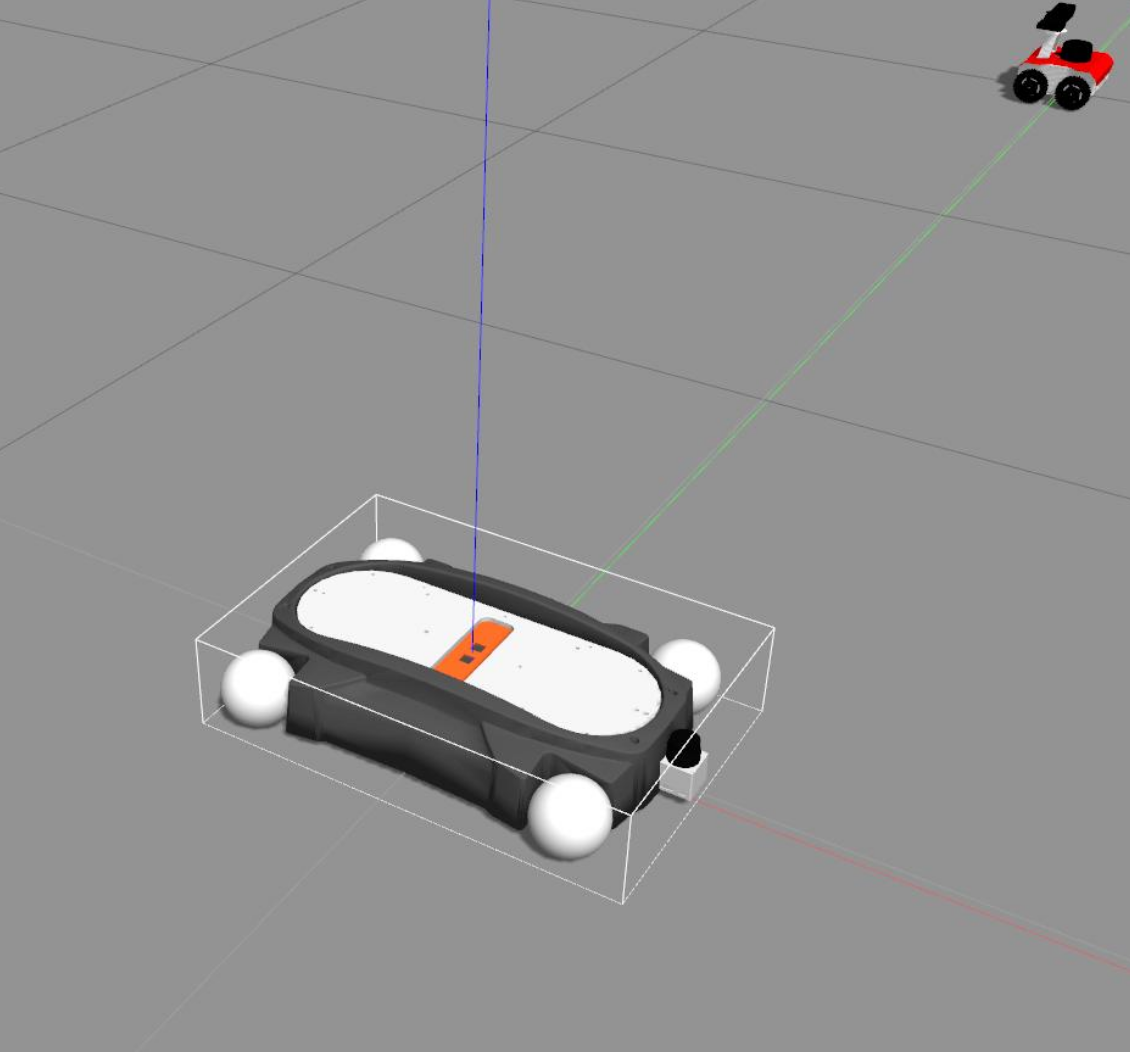
\includegraphics[width=\textwidth]{bot3}
        \caption{Youbot}
        \label{fig:bot3}
    \end{subfigure}
    \caption{Three commonly used robots with very different shapes and sizes.}
    \label{fig:bots}
\end{figure}

As an individual working in a cooperative operation, knowing the capabilities
of you and your teammates is necessary to the division of tasks. This idea
provides the basis for this proposed research. As homogeneous multi-robot systems
are inherently limited based on the capabilities of the specific robot,
it makes sense to venture down a heterogeneous avenue. A lot of research
has gone into heterogeneous multi-robot systems in the past few years, but a
common trend amongst most of them is that the model is built for the specific
platforms that are to be used. This proposed research is meant to provide the
groundwork for a heterogeneous model that allows for the insertion of a
robots with different skill sets with the purpose of enhancing the overall
capability of the system. This framework would allow for a variety of models
to be built on top of it, with a variety of hardware. Researchers wanting to
build a specific system could allocate funds and resources to build each member
to accomplish a portion of the overall task, possibly allowing for more cost
efficiency and remove unnecessary redundancy. The main challenge in this
research will be finding the optimal way to reassign tasks based on defined
capabilities of each robot in the system. This brings up a secondary, more basic,
challenge of defining robot’s characteristics in a simple yet comprehensive manor.
All-in-all, this research acts as a proof of concept for task division based on member
attributes, or individual robots capabilities, and will allow for a high degree of
heterogeneous utilization and multi-robot model expansion.

\begin{figure}[H]
  \centering
    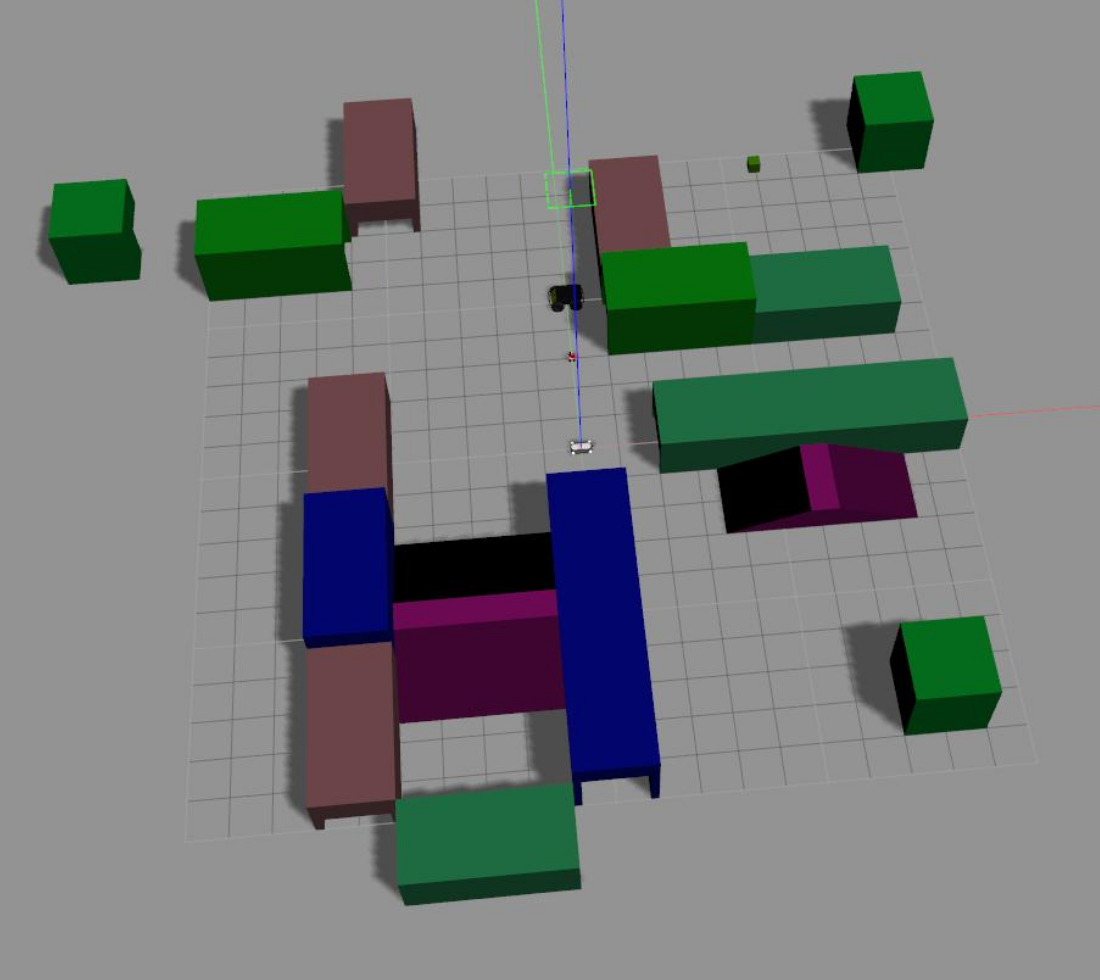
\includegraphics[width=0.5\textwidth]{map2}
  \caption{Gazebo map, with different terrain. Open terrain in gray, short tunnels in red and green, tall tunnels in blue.}
  \label{fig:map}
\end{figure}



\subsection{Algorithms}
For navigation we used two methods. The first is a Breadth First Search (BFS) which explores the cells adjacent to the robots
current positions, before exploring the second level of adjacent cells. After determinining explorable cells method getPath as described in Algorithm 1 will compute the a hueristic based on the manhattan distance to determine a set of cells that make up an optimal path. For robot exploration getPath can be called for exploration by simpling passing in a goal represented as the nearest unexplored node a summary of the path planning algorithm can be called with the goal being the nearest global unexplored node as shown in the algorithm in figure \ref{fig:a-star}.
The use cases for this method are as follows: a) robot needs to swap locations due to percieved danger, b) robot finds an obstacle (tunnel) it cannot explore and needs another robot to explore it 3) the robot's tree-state is not being beconed will return to performing exploration.
\begin{figure}[H]
 \centering
   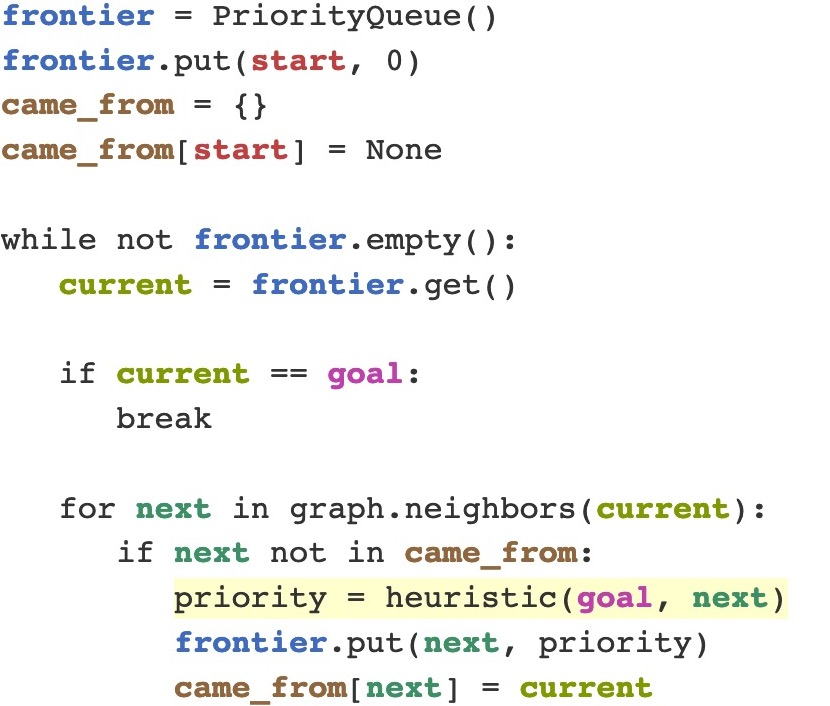
\includegraphics[width=0.5\textwidth]{a-star}
 \caption{An overview of the A* Algorithm \cite{a-star}} \label{fig:a-star}
\end{figure}


\subsection{Entities}
The Entity class is the base physical structure for this testing package. This could represent a static
or one of the two derived classes: Neighbor and Robot Entities hold major variables like state
information, initial position and odometry. The Neighbor and Robot classes are very similar to each other
as they both represent robots, the Neighbor class is just used to hold the information for the
Robot's neighboring robots as they do not need to keep track of their entire path and known map,
like they are doing for themselves.


\subsection{Steering}

The challenge using a centralized class stucture like the one proposed is the necessity to steer all robots in set
using a single set of steering methods. Each method was generalized to control a robot independent of its motion model. To achieve this
four steering methods were utilized, 1) goBackward(), goForward(), goRight(), goLeft(), turn(angle), face(goal). The idea is such that the robot locomotion would not be defined by a new set of steering methods, but instead would rely on
a different sequence of steering calls to perform the same motion. For instance, to turn right a differential robot like the rosbot
would call function goRight() followed by goForward(), while a holonomic robot would be ale to directly call goRight(). The robot motion attributes as described in table \ref{tabl:attributes} will be used to better tune this steering model.The addition of robot attributes could be added to a yaml file, uses and configuration of yaml files is briefly described in section Adding Robots. This simplified experiment focused on the youbot, husky, and rosbot. These robot locomotion models were far from idealistic which gave us a better testing platform for later porting on the physical platforms, but made experimentation challenging. In experiment the huskies linear and angular control actions were greatly impeded due to the frictional force induced on its large outdoor wheels, to mitigate this affect we overloaded the turn method to include a turn radius. In hindsight, we could have applied a gain factor to the turn method to provide a larger control input. Alternatively, the rosbot wasn't greatly effected by the frictional force when applying an angular velocity, however it did suffer from aggregate error, whereby the robot would divert from the direction of its input trajectory after some time. The youbot responded optimallly to the steering sequences, and would serve as a good candidate for beginner user testing and education in this framework.

\subsection{Adding Robots}
This framework allows for easy addition of robots by simply
adding the details for the new robot in the xml robots launch file. The mutlirobot launch file is called robots.launch
this xml sets up the robot models \ref{fig:bots}. This file calls .yaml which stores the data for the robot controller scripts, these files define the parameters needed for the motion models for each robot. This launch file also utilizes .xacro files which configures the robot form for use in the gazebo simulation environment and physics engine. To add any additional information
yaml files can be used to set rosparams and can be queried in any rosnode as long as the yaml file
was specified in one of the launch files as a rosparam. Utilization of the yaml files is essential
to adding and sharing information like hardware characteristics before Robots enter the main loop. So all in all, By configuring
the launch file with the proper robots, one can edit the one robot launch file to have each robot launch
any set of nodes that would exist in each robot's namespace.

One thing that was essential to streamline and allow for flexibility was the instantiation of robots via partitioned
launch files. By defining separate roslaunch files instead of one, it is easy to see where to
put new robots as well as ensure that one point of failure is taken care of.
The one robots launch file launches nodes that are to be in every robot,
who are defined by namespaces in the context of ROS. The robots launch file is where robot descriptions
are set along with locations of urdf files containing meshes and other simulation specific
data for the individual robot. The global multi-agent launch file used is hare sim.launch this file calls robots.launch this file calls one robot.launch which launches the hare node and spawns the robots in the gazebo simulator.


\subsection{Multi-Agent Testing Framework}
After exploring a set of options to test this idea, the best place to go was to the drawing
board. Taking a step back it was decided that pushing to get straight into hardware testing
was a poor decision and the underlying concept of heterogeneous task reallocation based on
capabilities needed to be tested at the lowest of levels. To do this, the creation of a testing
framework in roscpp was necessary. This framework allows for easy addition of robots by simply
adding the details for the new robot in the xml robots launch file. To add any additional information
yaml files can be used to set rosparams, just as was done here for robot capabilties. By configuring
the launch file with the proper robots, one can edit the one robot launch file to have each robot launch
any set of nodes that would exist in each robot's namespace. This allows for testing of a completely
decentralized algorithm in a centralized system. The reason this was done was because of the difficulty
of getting a multimaster architecture working within gazebo.
